%%
%% Class homework & solution template for latex
%% Matthew Gardner     
%%
\documentclass[twoside,11pt]{article}
\usepackage{amsmath,amsfonts,amssymb,amsthm}
\usepackage{graphicx,color}
\usepackage{verbatim,url}
\usepackage{listings}
\usepackage{upquote}
\usepackage[T1]{fontenc}
%\usepackage{lmodern}
\usepackage[scaled]{beramono}
%\usepackage{textcomp}
\usepackage{enumerate}
\usepackage{bm}
\usepackage{mathrsfs}

\usepackage[linesnumbered]{algorithm2e}	

% Directories for other source files and images
\newcommand{\bibtexdir}{../bib}
\newcommand{\figdir}{fig}

\newcommand{\E}{\mathrm{E}}
\newcommand{\Var}{\mathrm{Var}}
\newcommand{\N}{\mathcal{N}}
\newcommand{\matlab}{{\sc Matlab}\ }

\setlength{\textheight}{9in} \setlength{\textwidth}{6.5in}
\setlength{\oddsidemargin}{-.25in}  % Centers text.
\setlength{\evensidemargin}{-.25in} %
\setlength{\topmargin}{0in} %
\setlength{\headheight}{0in} %
\setlength{\headsep}{0in} %

\theoremstyle{definition}
\newtheorem{MatEx}{M{\scriptsize{ATLAB}} Usage Example}

\definecolor{comments}{rgb}{0,.5,0}
\definecolor{backgnd}{rgb}{.95,.95,.95}
\definecolor{string}{rgb}{.2,.2,.2}

\lstset{ % preferences
    frame=single,
    basicstyle=\footnotesize,
    keywordstyle=\bfseries\color{red},
    numbers=left,
    numbersep=5pt,
    showstringspaces=false, 
    stringstyle=\color{blue},
    tabsize=4,
    language=C,
    basicstyle=\small\ttfamily,
    %mathescape=true,
    emptylines=1,
    %showlines=true,
    %numbersep=5pt,
    breaklines=true,
    commentstyle=\color{comments},
    backgroundcolor=\color{backgnd},
    %keywordstyle=\ttfamily, \normalfont,
    showstringspaces=false
}
        
        
\newcommand{\matp}{\mathbf{\gg}}

\begin{document}

\centerline{\Large Homework 4 Problem 2 Report}
\centerline{Matthew Gardner (106880794)}
\centerline{ComSci 557}
\vspace{.2in}

My scene uses an image of New York City skyscrapers at dusk. My intention was to give it some specular light to emphasis the sunset and then to distort it with a unique noise map. The noise map I ended up making is a `grid' of a city taken from a satellite. The noise map emphasizes small details of roads and buildings, and my intention was have these details distinguishable in the distorted scene. 

\begin{center}\begin{tabular}{ccc}
	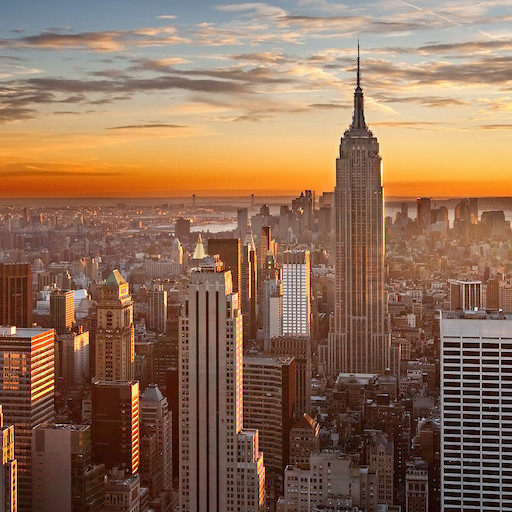
\includegraphics[width=.3\textwidth]{color-map_landscape} &
	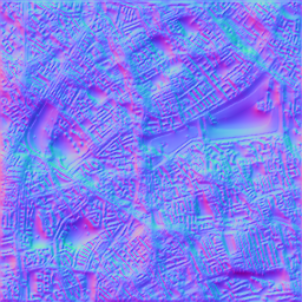
\includegraphics[width=.3\textwidth]{noise-map_city}\\
	Landscape (Color map) & Noise map
\end{tabular}\end{center}
I first observe results of some extreme displacement functions. When calculating a large noise vector by not scaling down the normalized value, or even by scaling it up, the details of the noise map are more visible in the scene. As shown in the figures below, you can make out the blocks of street as well as smooth parts of the noise map. At 5 times, the noise becomes too dense. 

\begin{center}\begin{tabular}{ccc}
	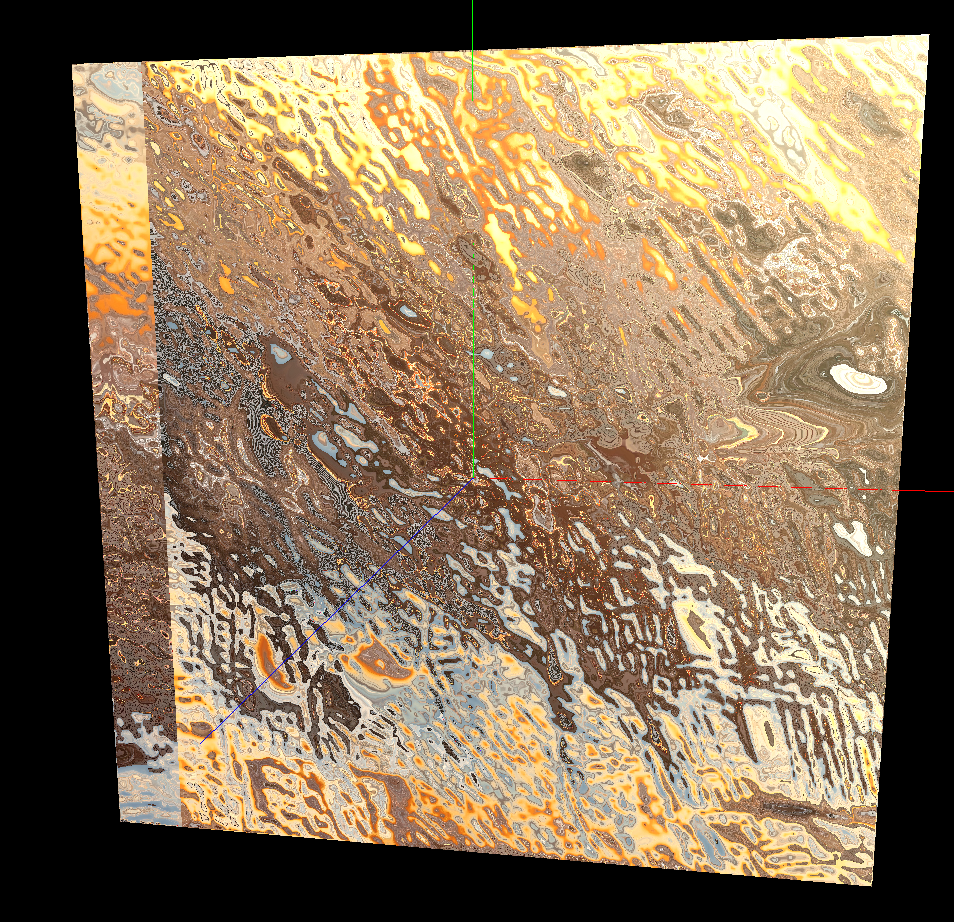
\includegraphics[width=.3\textwidth]{1x_normal_noise} &
	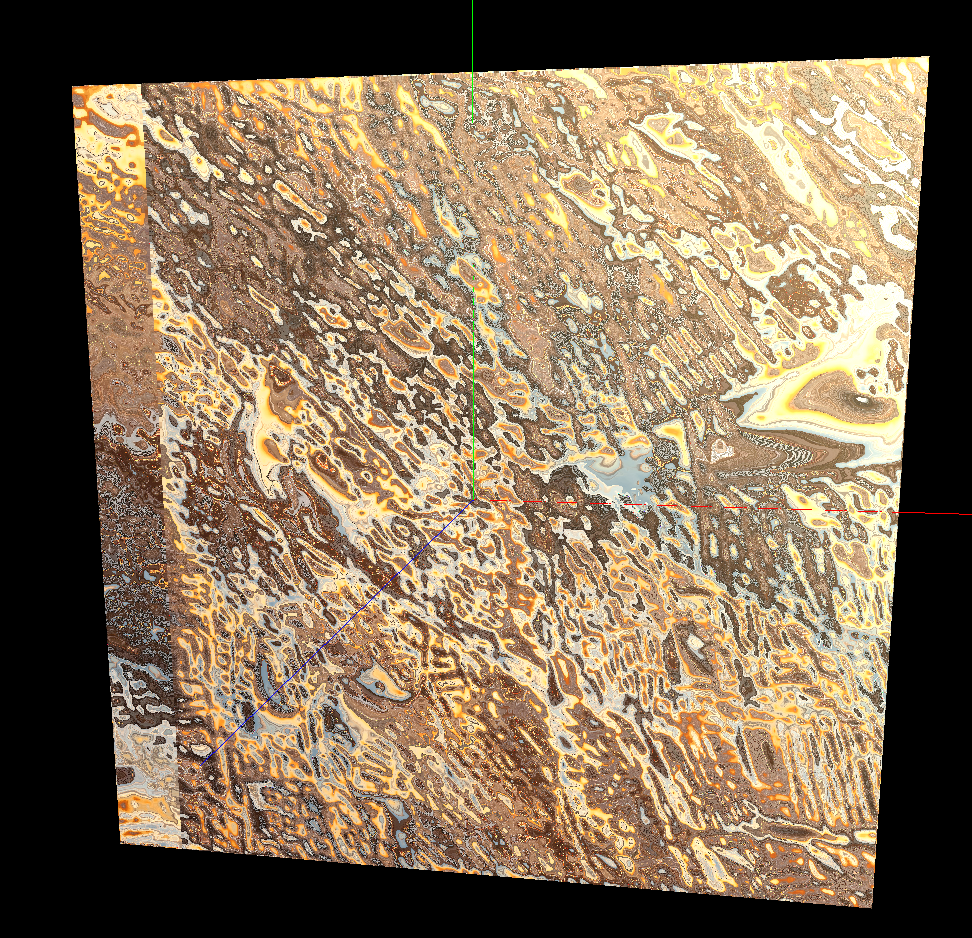
\includegraphics[width=.3\textwidth]{2x_normal_noise} &
	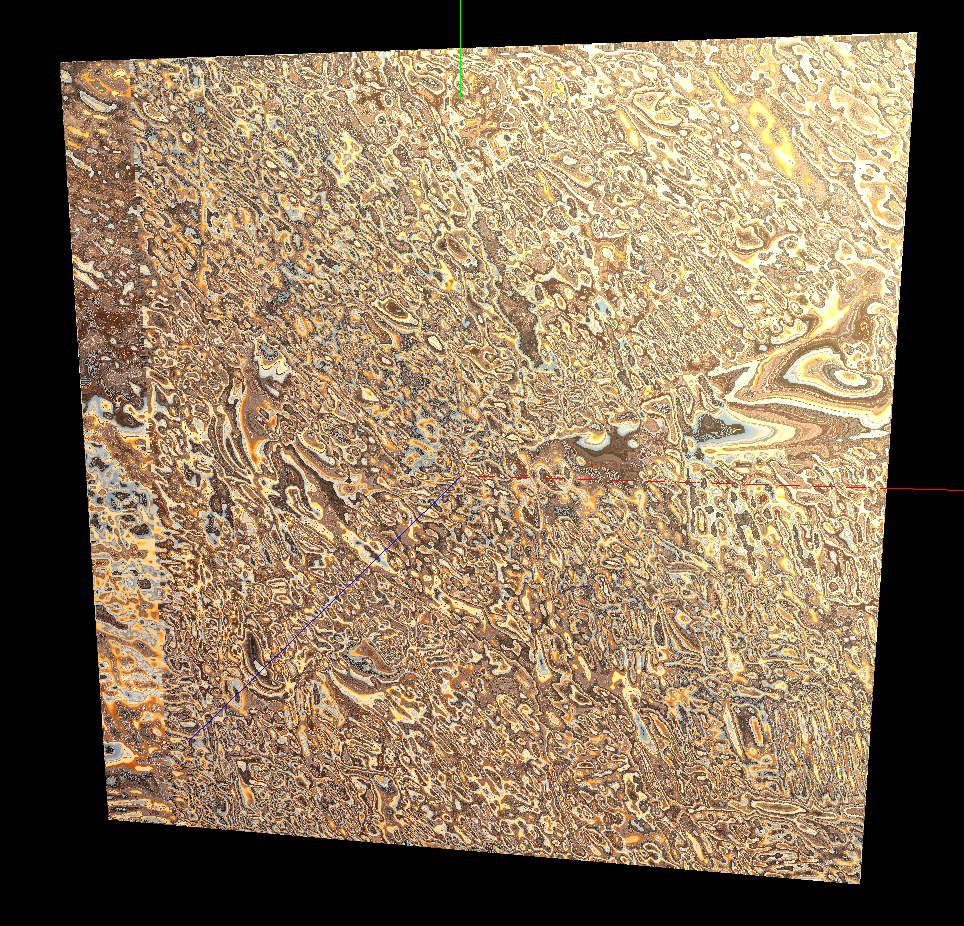
\includegraphics[width=.3\textwidth]{5x_normal_noise}\\
	$1\times$ Normalized Noise Vector & $2\times$ Normalized Noise Vector & $5\times$ Normalized Noise Vector
\end{tabular}\end{center}

Regardless, the result is undesirable because you can hardly see much of the landscape. My goal is to have the landscape still distinguishable, but with minimal displacement so you can just make out the noise map. Below are some results after scaling back the noise vector in different ways.

\begin{center}\begin{tabular}{ccc}
		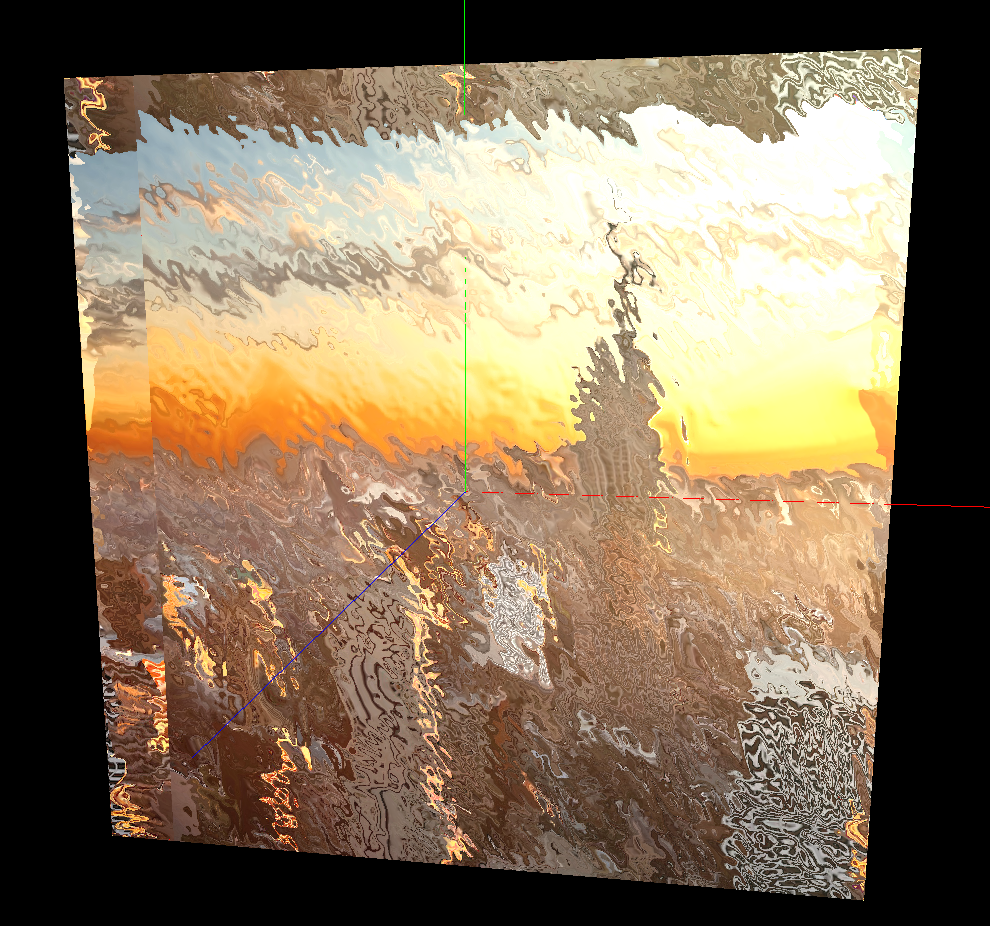
\includegraphics[width=.4\textwidth]{less_noise} &
		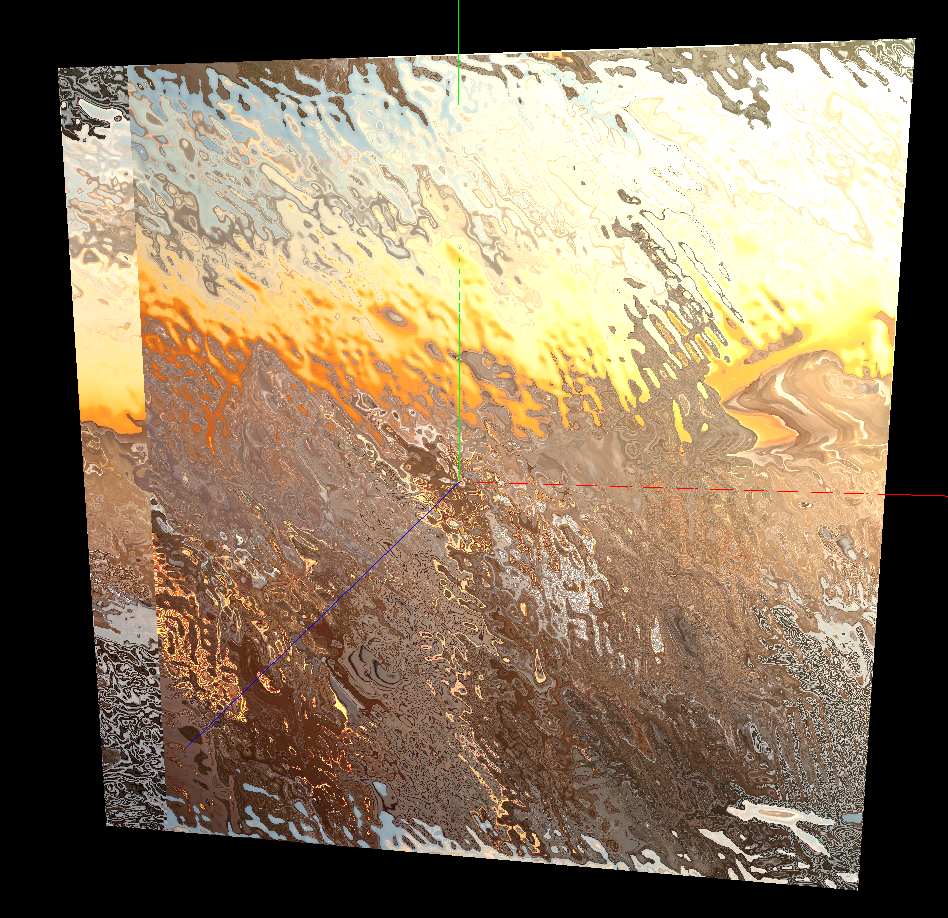
\includegraphics[width=.4\textwidth]{more_noise}\\
		Less noise & More noise\\
		$(\text{noiseVec} * 3.0 - 2.0) * .1$ & $(\text{noiseVec} * 5.0 - 0.0) * .01$
\end{tabular}\end{center}

It proved difficult to make the high level of detail in the noise map to be visible when mixed with the color information of the landscape. Colors of the landscape give off a sense of depth and size that conflict with the displacement. This often lead to what looks like the reflections of landscape in rippled water. When combined with the specular light, this unintentional result turns out to look pretty nice.

\end{document}
